In the previous section, we have already described some features that could also provide useful in a cross-device testing scenario. Those features include:
\begin{itemize}
	\item Refreshing all devices/Loading a URL on all devices
	\item Device Emulation
	\item Testing on Real Devices
	\item Recording and replaying interactions
	\item Many features that are already included in browser developer tools
\end{itemize}

While some of those features like refreshing all devices are already very useful in cross-device testing scenarios and can be adopted without much adjustment, other features like device emulation still have some limitations that make them difficult to use for cross-device testing and have to be extended in some ways. In the following subsections, we will describe the core concepts of our system and how we adapted existing features to suit the needs of cross-device testing.

\section{Emulation of Multiple Devices}

Device emulation is already often used for testing responsive websites. In its simplest form, device emulation can just be done by resizing a browser window so it looks and feels like a smaller device. However, manually resizing a browser window such that it has a resolution that is typical for actual devices is difficult. Furthermore, just emulating the screen size is not enough to realistically emulate a real device: Mobile devices typically use touch interactions and often have poor network connectivity. Those limitations have led to the emergence of more sophisticated tools for device emulation. Advanced device emulation facilities like the Device Mode in Chrome DevTools emulate different screen sizes, touch capabilities, network conditions, as well as location and acceleration sensors. They also typically provide a list containing a large number of existing devices, thus realistic resolutions can be emulated. However, all those tools have one common limitation: They can emulate only one device per browser tab or window. Another limitation of those tools is that even when multiple browser windows are used, those browser windows share their local resources such as local and session storage. This limits the use of those tools for cross-device applications, as cross-device applications usually run on multiple independent devices and thus should not share any local resources. To accurately simulate the use of a cross-device application in real life, some mechanism for preventing devices from sharing local resources is needed. Nowadays, there are several possibilities for doing this: First, different browser profiles can be used in different browser windows. Second, the incognito mode provided by browsers can be used to prevent sharing of local resources. Lastly, multiple independent browsers can be used. However, those solutions all have some limitations: Using multiple independent browsers limits the number of devices that can be emulated to a rather small number. Furthermore, all of those solutions require multiple windows that need to be arranged somehow and tasks like creating multiple profiles might be time-consuming and not what the developer wants. This is tedious and frequent switching between browser windows is required. Additionally, if the developer actually wants to use browser debugging tools, those tools have to be opened in all different windows which requires a lot of space and also limits the number of devices that can realistically be emulated. The screen size of the device that is used for emulating the devices can also be a limitation in other scenarios: If the device has a full HD screen but wants to emulate a full HD device as well as some mobile devices simultaneously, those devices cannot be ordered such that all devices are visible at the same time. The developer would have to put one window in full screen. This would make switching between devices even more tedious and the consequences of the interactions performed on the full HD device could not be seen in real-time because the developer would have to switch to the other windows first. Also, things like emulating a 4K TV are impossible on a device with a smaller resolution. 

Those limitations all contribute significantly to the difficulty of cross-device application testing. Using these limitations, we gathered a number of requirements for device emulation in our system:
\begin{itemize}
	\item It should be possible to emulate multiple devices in one browser window.
	\item The emulated devices should not share any local resources.
	\item The screen size should not be a major limiting factor concerning the number of devices that can be emulated simultaneously.
	\item The developer should have access to a list containing some existing devices.
\end{itemize}

Our system provides a solution that fulfills all those requirements. Firstly, the user can add multiple emulated devices simultaneously. The developer can either select the emulated devices from a list of existing devices or create a custom device. The user can create a custom device just for one-time use, or they can save it to the list of existing devices for later use. This allows developers to quickly extend the devices they have access to with new devices. Devices can essentially be assigned to one of four categories:
\begin{itemize}
	\item Desktop devices: For simplicity, this category includes desktop PCs as well as laptops.
	\item Tablets
	\item Mobile phones
	\item Wearables
\end{itemize}
Although some devices may not easily be classified, e.g. 2-in-1 devices that can either be used as a tablet or laptop by just plugging in a keyboard, those categories give a rough overview of the types of different devices. This categorization of devices also makes it easier for developers to emulate different types of devices without having to know any exact device names. By just adding some devices from each category, the developer can make sure that a very large range of devices is covered, as devices in the same category typically have similar properties such as screen size and input modalities. Our list of existing devices includes multiple devices from each of those categories. For the desktop devices, we just provide some typical resolutions of desktop PCs and laptops. The list of tablets and mobile phones includes most of the well-known devices in that area. The list of wearables so far only includes some smart watches, as most other wearables do not have access to a modern web browser (yet).

Once the developer has created an emulated device, they can move it to the desired location on the screen. Instead of ordering devices automatically, we chose to give the developer the freedom to choose how to place the emulated devices. This makes it easy to accurately simulate specific scenarios, e.g. a presentation room where two large screens are placed next to each other. To conquer the challenge of limited screen size, all emulated devices can be scaled up and down. Scaling a device does not change the resolution of the device and thus has no influence on the look of the application. This allows the developer to scale down an emulated device and have more space available for devices. If the developers has difficulties performing an interaction on a device because it is scaled down, they can just scale it up again. However, dynamically changing the resolution of an emulated device is also possible. Thus, the developer can continuously increase or decrease the resolution of the device to immediately see how the application looks with different resolutions. Figure~\ref{fig:difference_resizing_scaling} illustrates the difference between resizing a device and scaling a device using W3School's website\footnote{\url{http://www.w3schools.com/}}.

\begin{figure}[H]
  \centering
    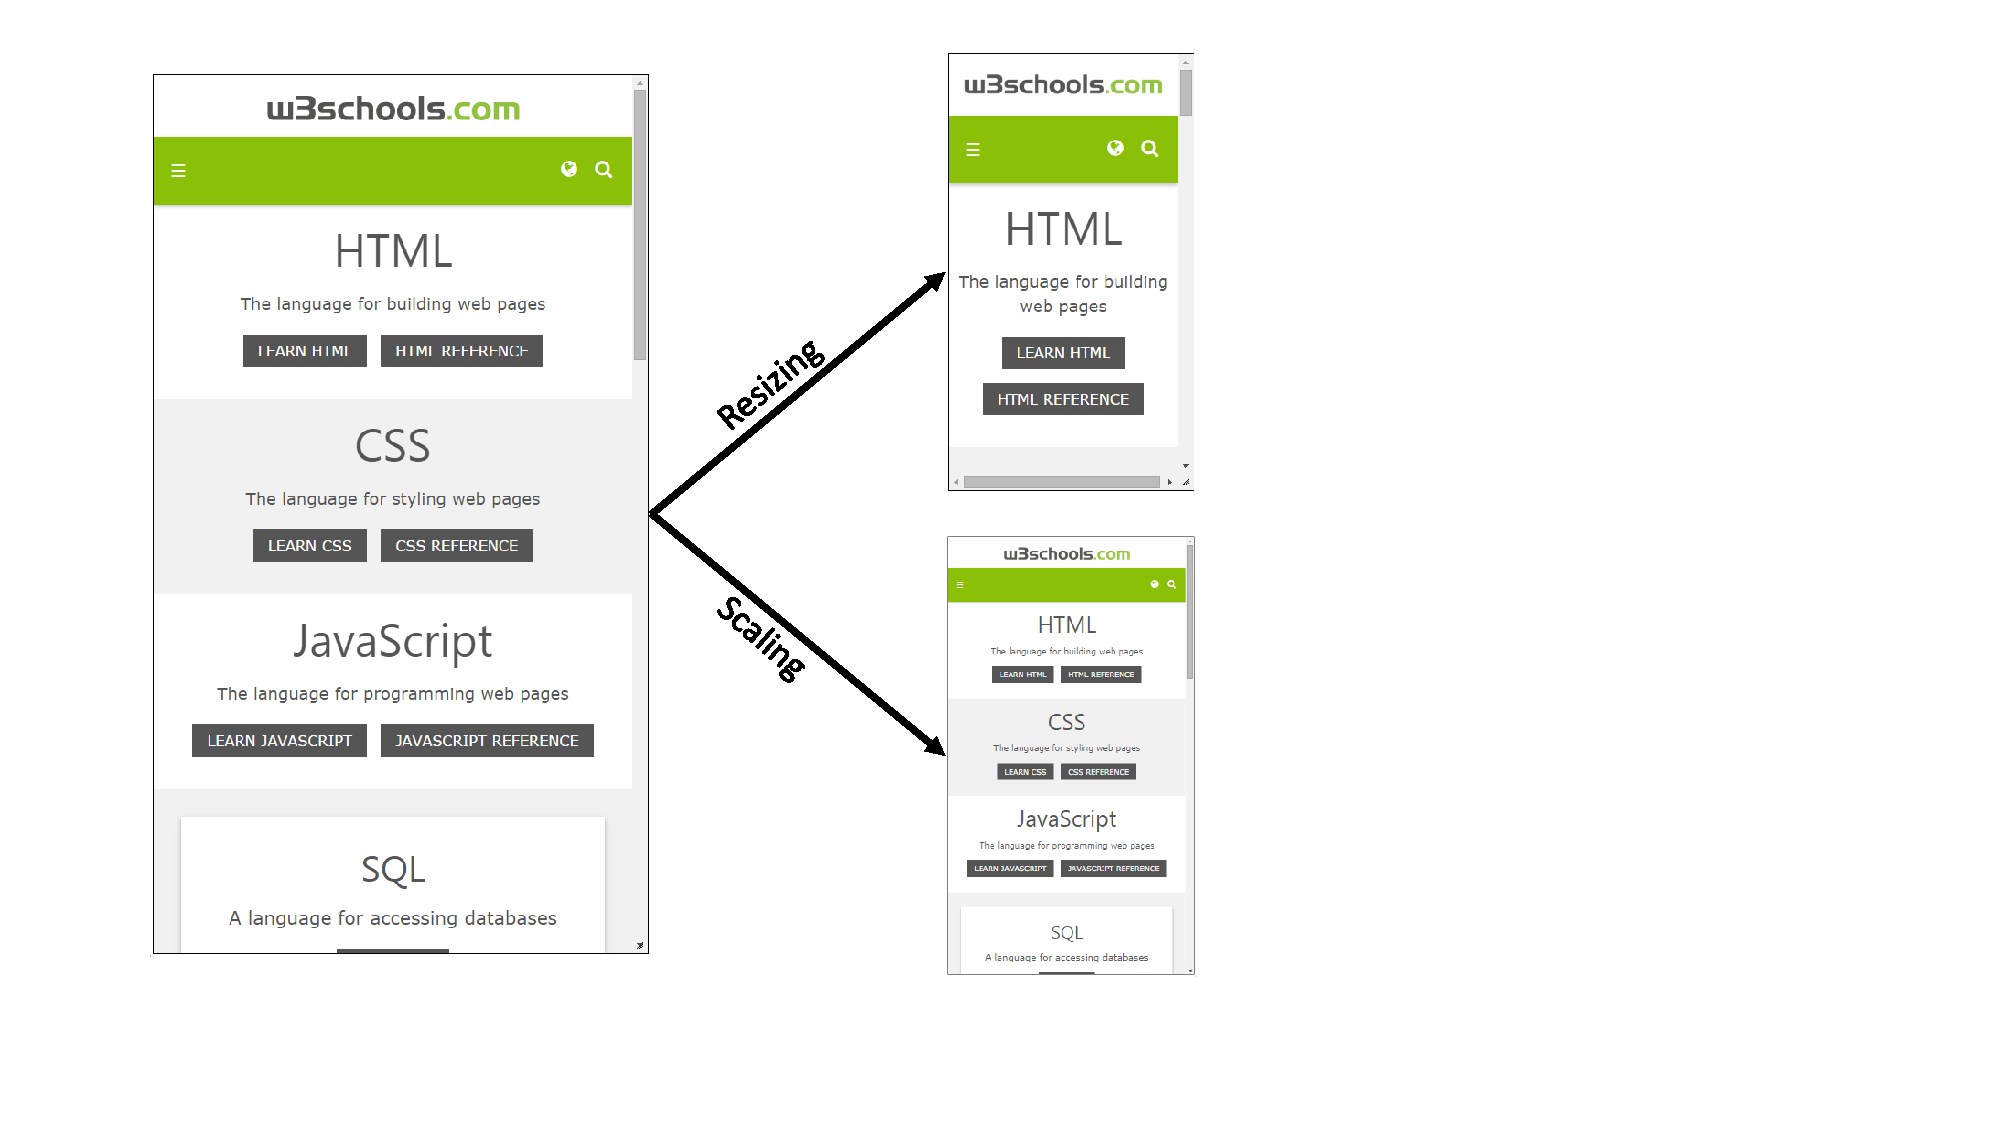
\includegraphics[width=1.0\textwidth]{images/difference_scaling_resizing.pdf}
	\caption{Difference between resizing and scaling a website}
	\label{fig:difference_resizing_scaling}
\end{figure}

Finally, our system includes a mechanism that prevents the sharing of local resources between emulated devices. In summary, our system allows the developer to create multiple emulated devices with just a few clicks and to order the devices as needed for the application that the developer wants to test. There is no need for constant switching between multiple browser windows and creating new browser profiles. Also, the developer tools can just be opened for the browser window where all devices are emulated instead of having to open them for each emulated device.
 
\section{Easy Integration of Real and Emulated Devices}

Emulating devices is a versatile tool for testing cross-device applications on many different devices. However, it does not completely eliminate the need for testing on real devices: Device emulation is always limited to certain aspects that are being emulated, e.g. screen size, resolution, touch interactions, location, and more. However, not every little detail of a real device can be emulated accurately. The following list provides an overview of some of the limitations regardinf testing on emulated devices:
\begin{itemize}
	\item Touch interactions: Even though modern device emulators can also emulate touch interactions, performing a gesture with the mouse will never feel the same as the actual touch interaction. An interaction that works great with the mouse might feel awkward when performed on a real device and vice-versa. Also, multi-touch interactions such as pinching are difficult to emulate realistically on an emulated device.
	\item Interrupts: While using an application on a real device, the user might be interrupted by things like the arriving of a text message. Those interrupts cannot be simulated in a realistic way on an emulated device.
	\item Performance: A desktop PC typically has much more computing power than a mobile device. If an application uses too much performance for most mobile devices, this might not even be noticed if the developer only test on emulated devices.
	\item Display: The display quality and thus also the look of an application varies greatly depending on the device. Only emulating devices on a desktop PC cannot account for those differences in display quality. 
	\item Sensors: Modern devices have a large number of different sensors that cannot all be emulated realistically. One particular problem is the orientation of the device: A user might switch between landscape mode and portrait mode on purpose or accidentally at multiple points. Although the orientation of emulated devices can also be switched, this does not accurately simulate the behavior of a real user.
\end{itemize}
Although this list gives a good overview of the differences between real and emulated devices, this list is by far not complete and what happens on a real device cannot always be foreseen by testing on emulated devices. Thus, testing on real devices is crucial for the successful development of a cross-device application. 

The importance of testing on real devices leads to a new requirement for our system: It should easily be possible to connect real devices to our system. QR codes have become increasingly popular over the last few years and almost all devices nowadays are equipped with at least one camera. Thus, our system provides a QR code that can be scanned with real devices to connect them to our system. This makes it easy and efficient to connect a large number of real devices to our system. As a backup mechanism, the developer can also type a URL into the browser of a real device to connect it to our system. Once a real device is connected to our system, it is represented with a proxy and can be used in the same way as an emulated device. The developer can also use emulated devices alongside real devices if desired. Thus, our system allows the user to test their application on only emulated devices, only real devices, or both at the same time. This flexibility makes it easy to test a large number of different scenarios.

\section{Easy Switching of Device Configurations}

Cross-device applications are typically not always used by the same users and with the same set of devices. The same user may sometimes use their mobile phone and laptop simultaneously and at other times only their mobile phone or tablet. Thus, the number of devices using a cross-device application and their characteristics may vary greatly. Depending on those devices, the UI distribution might be different. A cross-device application needs to be able to support all those different device scenarios. However, some cross-device applications are also targeted to specific scenarios, e.g. a presentation room with multiple big screens that are always present, in addition to some mobile devices that are only in the room when their owner is attending a presentation. In such an application, the developer would probably want to emulate the devices that are always present when the application is used whenever they are testing the application. Thus, it is a requirement for our system that multiple different device scenarios can quickly be created. 

Our system allows the developer to create a device configuration, save it for later, and then re-use it. A device configuration consists of the following information:
\begin{itemize}
	\item The number of emulated devices.
	\item The types of the devices.
	\item The position and scaling of the devices.
\end{itemize}
Thus, the developer can easily re-use device configurations without much effort and switch between different device configurations efficiently. Thus, testing a cross-device application in many different device scenarios can be done without much effort. A user can just load one device configuration, try out the application and switch to the next device configuration if everything works as expected. The developer can also create a device configuration where only the static devices are saved in the configuration, e.g. in the example mentioned above, the developer could create a device scenario where only the big screens are already configured and then dynamically add some mobile devices to create a more realistic scenario.

\section{Integration with Debugging Tools}

Many of the features integrated into the debugging tools of browsers are also immensely useful for testing cross-device applications, some might be even more useful for testing cross-device applications than for testing traditional web applications. However, those tools are typically limited to debugging one device at a time. In our system, multiple devices are emulated in the same browser window. While this simplifies some ways of debugging multiple devices, e.g. because messages logged from all devices are shown in the same console, it makes other things more difficult, such as trying out things in the console by sending commands. Google Chrome allows the developer to switch between different frames in the console and thus address different frames with commands, but it is not always obvious which frame corresponds to which device. Also, the developer might want to try out the same thing on multiple devices and would have to switch between multiple frames to address all devices. Furthermore, even though logging messages from all devices are displayed in the console, there is no way of knowing which device sent the message. This further complicates the debugging of cross-device applications. The same limitation applies to JavaScript errors that are also shown in the console, but can not easily be related to a device. Further limitations of the browser-included debugging tools are that navigating to the HTML of an emulated device can be rather tedious, that CSS can only be applied to one device at a time and that function breakpoints can only be added on one device at a time. Especially the last limitation can make cross-device application testing difficult because different devices have different responsibilities and not all devices might use all JavaScript functions. Consequently, adding a breakpoint inside a function on one device might not help with debugging the function at all, because the function is not even called on that device. The existence of real devices complicates things even more. By connecting the device to the desktop PC via cable, the developer gets access to remote debugging in Google Chrome. Remote debugging provides the same debugging tools as the normal DevTools, but it gets even more difficult to debug multiple devices at the same time. The remote debugging of each device is opened in a new window, thus the developer once again has to navigate between multiple windows. Also, getting an overview of all logging messages from all devices and sending commands to multiple devices becomes even more difficult. Despite those limitations, a tight integration with browser debugging tools is clearly desirable: Most of those tools have been around for quite some time and thus are already well tested and have gone through a series of improvements. Also, almost all web developers have already used those tools for extensive testing and are thus already familiar with them. From this, we can derive the following requirements for our system:
\begin{itemize}
	\item Logging messages should all be aggregated in one place and the device the messages originated from should also be easily identifiable.
	\item JavaScript errors should also be aggregated and be easily identifiable.
	\item It should be possible to send JavaScript commands to multiple devices at a time. 
	\item It should be easy to inspect the HTML of a specific device.
	\item It should be possible to add CSS to multiple devices at the same time (see Figure ~\ref{fig:css_aggregation}).
	\item It should be possible to add breakpoints to multiple devices simultaneously.
	\item If possible, all of the above requirements should also be applied for real devices.
\end{itemize}

\begin{figure}[H]
  \centering
    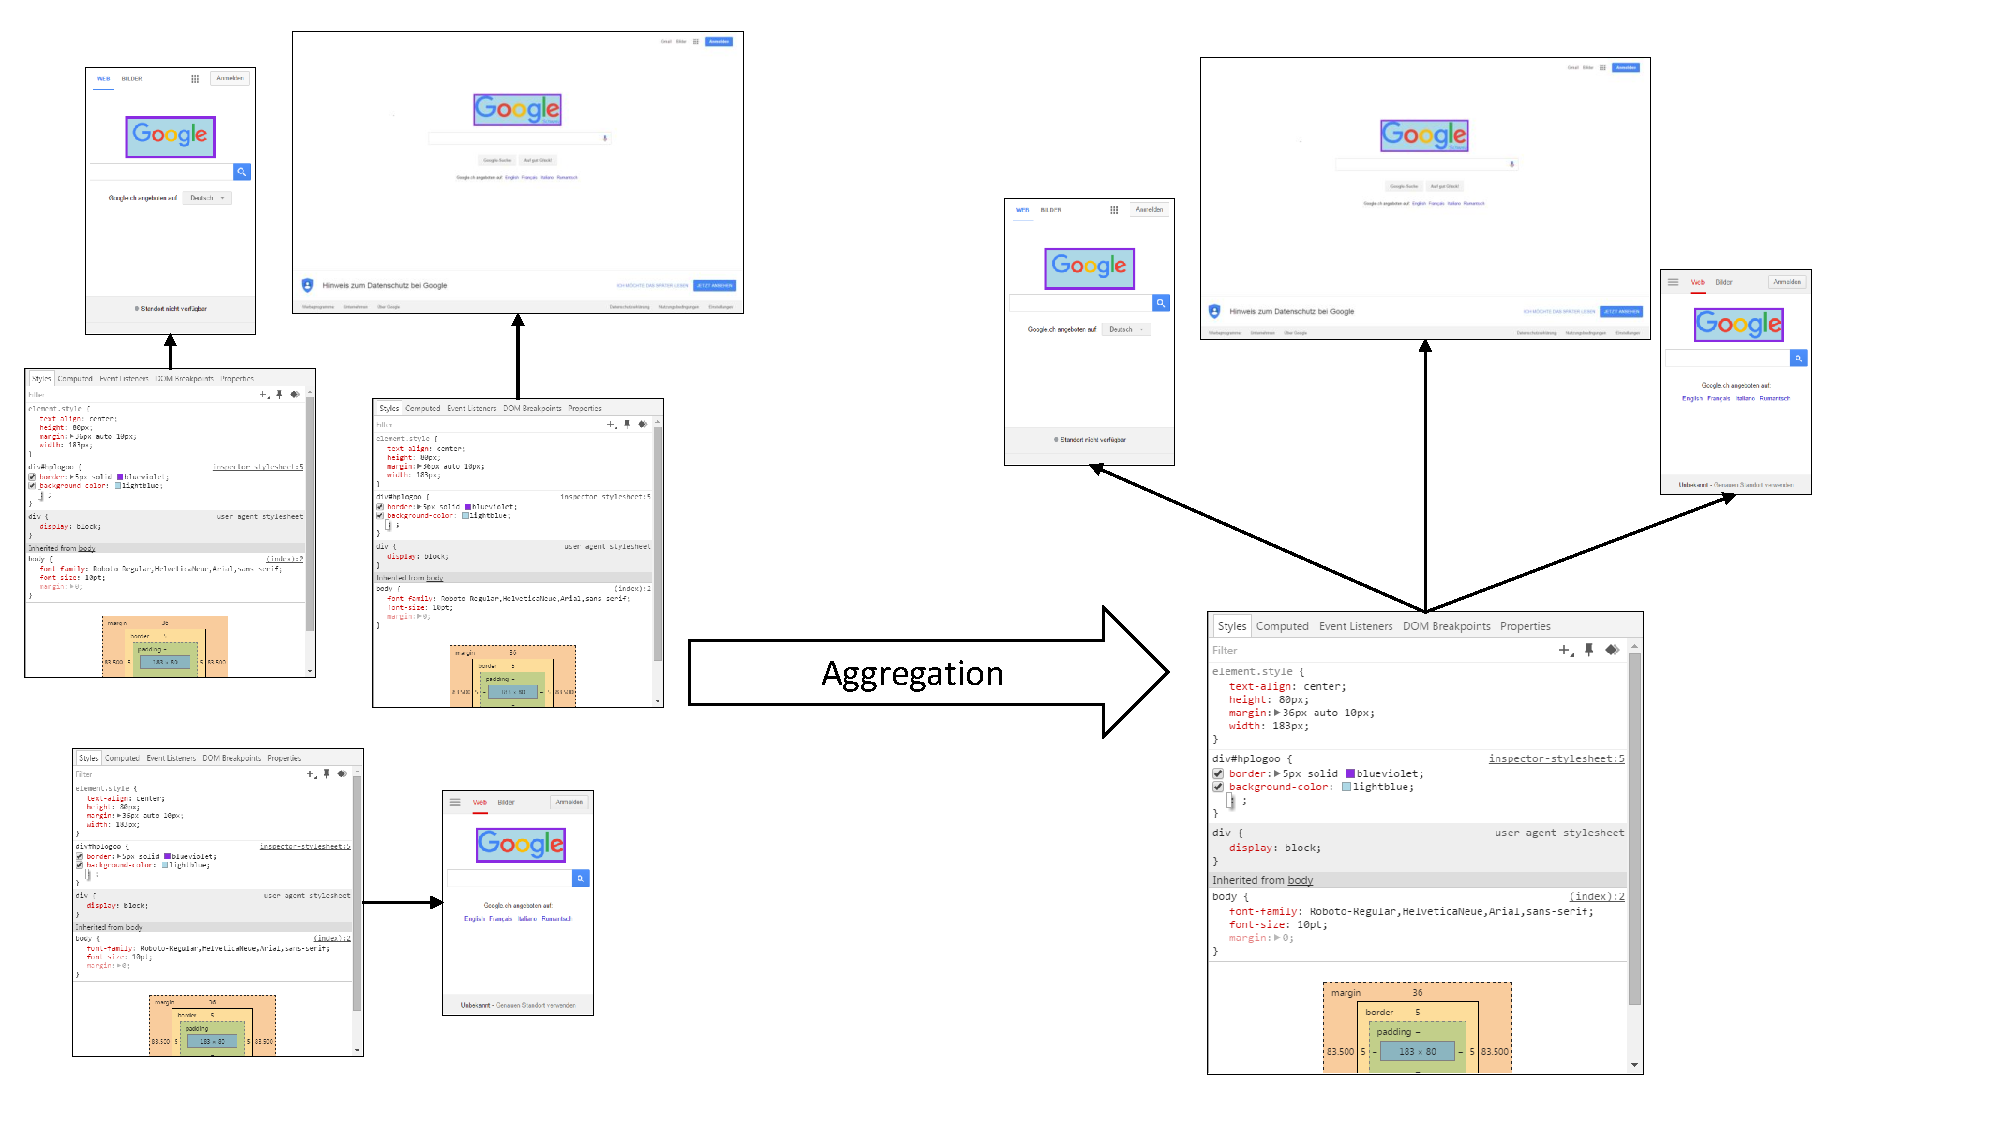
\includegraphics[width=1.0\textwidth]{images/css_aggregation.pdf}
	\caption{Editing CSS once for all devices}
	\label{fig:css_aggregation}
\end{figure}

Unfortunately, it is not feasible to extend the console of Chrome DevTools due to technical limitations. For this reason, our system includes its own JavaScript console. Each emulated and real device forwards all logging messages and JavaScript errors to our system. This allows us to aggregate all console outputs in our custom console. For easy identifiability, each device gets its own unique color when created and all console outputs are color-coded in the color of the device the output stems from. This color-coding makes it trivial to identify the device a message or error originated from. The large number of messages that are displayed in the console due to the larger number of devices makes it a key requirement that there are some ways of filtering messages. The developer can either filter the messages by type (error, warning, logging message, info), by content, or by device. Our console also allows sending commands to multiple devices. The developer can either send a command to all devices or they can deactivate some devices and only send the message to a subset of devices. Being able to send a command only to a subset of devices is important in a cross-device setting because some commands might only make sense on some devices and executing them on all devices could lead to potential errors or a decrease in performance. The return values of commands are also displayed in the console, again color-coded to match the device they came from. Thus, otherwise complicated tasks like checking the value of a global variable become trivial. Our custom console works exactly the same for emulated as well as real devices. This aggregation of console outputs from both emulated and real devices at least partially eliminates the need for remote debugging.

Modifying the browser-internal CSS editor such that it adds CSS to multiple devices is not feasible, just like with the JavaScript console. Thus, we also included a custom CSS editor with our system. The CSS editor is designed to feel similar to the CSS editors typically provided by browsers. Thus, the developer can specify a selector and then add some rules that are applied to HTML elements that match the selector. Again, the developer can either select all devices or a subset of devices. The CSS rules are applied to emulated devices as well as real devices. All CSS rules can be deactivated and activated again, edited, or removed completely. This allows the developer to quickly change the CSS of multiple devices and immediately see the result on all those devices. This is considerably less effort than adding rules to all devices individually or editing the CSS file, saving it and reloading all devices multiple times.

Additionally, our system also allows developers to add breakpoints at the beginnings of functions on all devices or a subset of devices. Breakpoints can easily be added by adding the name of a function to a list of functions that the developer wants to debug. The breakpoints are then automatically added to all activated devices. The developer can also easily inspect the function by clicking on a button. Furthermore, as soon as the functions that the developer is debugging are called on any device, the device where the function was called is highlighted. This makes it easy to identify the device that is currently being debugged. Unfortunately, this feature is limited to emulated devices. The JavaScript files of real devices cannot be accessed from within the browser debugging tools without remote debugging, thus adding a breakpoint to a JavaScript function of a real device is impossible from within our system. 

Finally, our system allows the developer to directly jump into the HTML of an emulated device just by clicking a button. Clicking this button navigates through the DOM of our system right into the body element of the emulated device. Again, it is technically impossible to implement this feature for real devices, just like with JavaScript debugging.

\section{Automatic Connection Management}

In order to use multiple devices in a cross-device application, those devices need to be paired with each other in some way. The mechanisms for pairing devices differ between different cross-device application frameworks: With some frameworks, all devices that open the cross-device application are paired implicitly. In other frameworks, for example XD-MVC, devices can be paired by copying the URL from one device to the other devices that should be connected. Other frameworks have more complicated mechanisms for connecting devices. In Connichiwa, one device runs a local web server and uses Bluetooth to detect nearby devices. The device then sends the IP of the web server over Bluetooth, enabling the other devices to access the received IP in a web browser. All of those three mechanisms have one thing in common: Devices are connected by opening a specific URL in the browser. However, other ways of connecting devices are also feasible: Some frameworks provide a function that can be called from a device to connect the device to another device by passing the ID of the device the device should be connected to. Also, many of the papers describing cross-device application development frameworks do not describe how devices are connected. Finally, cross-device applications can also be implemented independently of any framework and might use even more different ways for connecting devices. Thus, it is impossible to derive all ways in which devices could be connected in a cross-device application.

However, if the developer wants to debug a cross-device application, re-connecting the devices every time a new device configuration is used or possibly even when devices are refreshed is tedious and time-consuming. Thus, it is desirable that devices can be connected automatically. In order to achieve this, our system provides a custom connection function that can be implemented by the developer. Since the developer probably knows how devices are connected in their application, implementing this function should be trivial. Once this function is implemented, a device can be connected to another device by selecting the device to connect to from a drop-down menu. Furthermore, the developer can choose to automatically connect all newly added devices to an existing device session. Thus, connecting devices to each other becomes an easy task that can be achieved with just a few clicks.

\section{Coordinated Record and Replay}

Record and replay has already been used previously for recording and replaying user interactions in traditional web applications and especially AJAX web applications. The non-deterministic and asynchronous nature of web applications contributes much to the value of recording and replaying interactions in web applications. When a bug is encountered during web application testing, it is often difficult to determine the exact steps for reproducing the bugs. Reproducing bugs becomes even more difficult in cross-device scenarios where multiple devices are involved and the interactions performed on one device have some implications on other devices as well. Also, cross-device applications are often used by multiple users at the same time and it is difficult for the developer to simulate multiple users interacting with their devices simultaneously. Thus, we believe that record and replay can benefit cross-device application developers even more than developers of traditional web applications.

Our system allows the user to start recording interactions on a device at any time. Once, recording has started, the developer can perform the desired interactions on the device. After finishing recording, the interactions can be replayed on the same device, moved to other devices, or saved for later.  Furthermore, event sequences can be cut into multiple parts. The timing of the replays can be configured arbitrarily by dragging and dropping event sequences. This allows the developer to configure replays in many different ways: They can be executed in parallel, one after another, or anything in-between. The replays can then be started on all devices simultaneously. This makes it easy to simulate multiple users and devices in a cross-device environment. Since the events contained in an event sequence are performed by a real user, i.e. the developer, the timing of the individual events in an event sequence is very realistic. The developer can also breakpoints at a certain point of time. As soon as all events that occur before this point of time have been replayed, the replaying pauses and the developer can inspect the state of the devices. Thus, if the developer sees that after some events something goes wrong in the application, they can set a breakpoint, replay the events again and see what went wrong. The developer can also add breaks of one second between events to delay all following events. This allows the developer to spend some more time looking at the application before the replaying continues without having to set breakpoints. 